\documentclass[serif,mathserif,14pt]{beamer}
%\setbeamercovered{transparent}
\usepackage{listings}
\usepackage{amsmath, amsfonts, epsfig, xspace}
\usepackage{pstricks,pst-node}
\usepackage{multimedia}
\usepackage{beamerthemesplit}
\usetheme{chaosgroup}
% add bulgarian support
\usepackage[utf8]{inputenc}
\usepackage[english,bulgarian]{babel}
\usepackage[T2B]{fontenc}
% include subfigure package
\usepackage[normal,tight,center]{subfigure}
\setlength{\subfigcapskip}{-.5em}

\usepackage{animate}

%4 people are authors - \author[Bruce Wayne]{Bruce Wayne \quad Clark Kent\\Peter Parker \quad Alan Scot}
%\addtobeamertemplate{title}{\vskip-0.5ex}{}
\author[Йордан Маджунков]{Йордан Маджунков}
\title[Монте Карло\hspace{2em}\insertframenumber/\inserttotalframenumber]{Въведение в Монте Карло}
%\institute{ 
\includegraphics[width=5cm]{chaoslogo_white.png}}
\date{24 Октомври 2015} %leave out for today's date to be insterted

\usebackgroundtemplate {
\includegraphics[width=\paperwidth, height=\paperheight]{background.jpg}}
\defbeamertemplate*{title page}{customized}[1][] {

\setbeamercolor{author}{fg=write}
\vspace{5cm}
\begin{center}
\usebeamerfont{title} \Large \inserttitle\\
\end{center}
\begin{center}
\usebeamerfont{author} \small \insertauthor
\end{center}

}


\begin{document}

\maketitle

%\section{Introduction}  % add these to see outline in slides
\addtobeamertemplate{frametitle}{\vskip-0.5ex}{}
\setbeamertemplate{background canvas}[vertical shading][bottom=bottomcolour, middle=middlecolour, top=black]
\begin{frame}
  \frametitle{Въведение}
  Монте Карло алгоритми\pause
  \begin{itemize}
  \item Използват псевдо случай числа\pause
  \item Изчисляват приближено решение\pause
  \item Контрол на точността\pause
  \item Контрол на времето за изпълнение %leave out the \pause on the final item
  \end{itemize}
\end{frame}

\begin{frame}
  \frametitle{Мотивация}
  \pause
  Защото работи\pause
  \begin{itemize}
  \item с ограничени ресурси\pause
  \item върху сложни проблеми\pause
  \item в истинският свят\pause
  \item без алтернатива
 %leave out the \pause on the final item
  \end{itemize}
\end{frame}


\renewcommand*{\thesubfigure}{}
\begin{frame}
  \frametitle{История}
  \pause
  \begin{figure}[t]
    \centering
    \subfigure[Stanislaw Ulam]{
    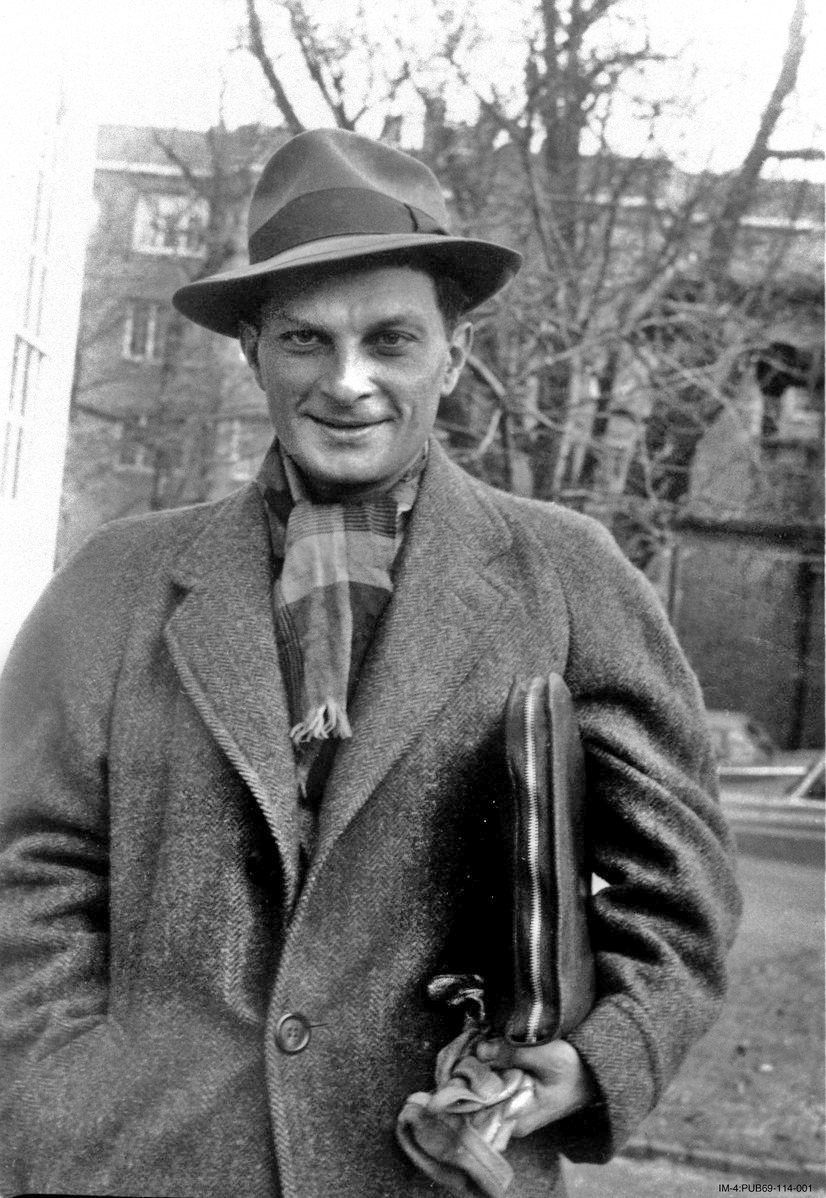
\includegraphics[height=6.0cm]{StanislawUlam.png}}
    \pause
    \subfigure[John von Newmann]{
    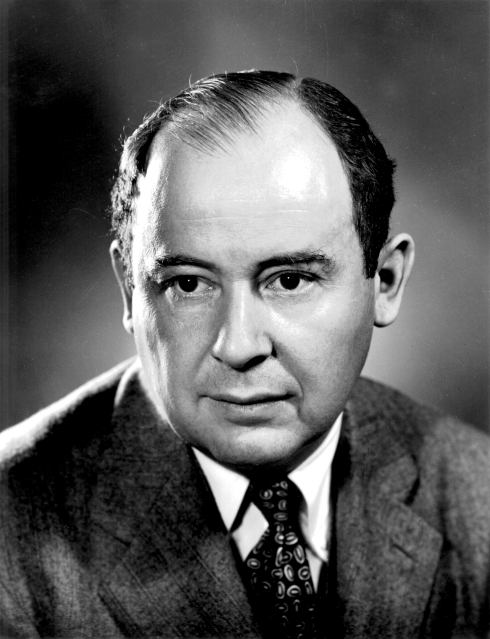
\includegraphics[height=6.0cm]{JohnvonNeumann.png}}
  \end{figure}
\end{frame}

\begin{frame}
  \frametitle{История}
  \begin{figure}[t]
    \centering
    \subfigure[Electronic Numerical Integrator And Computer]{
    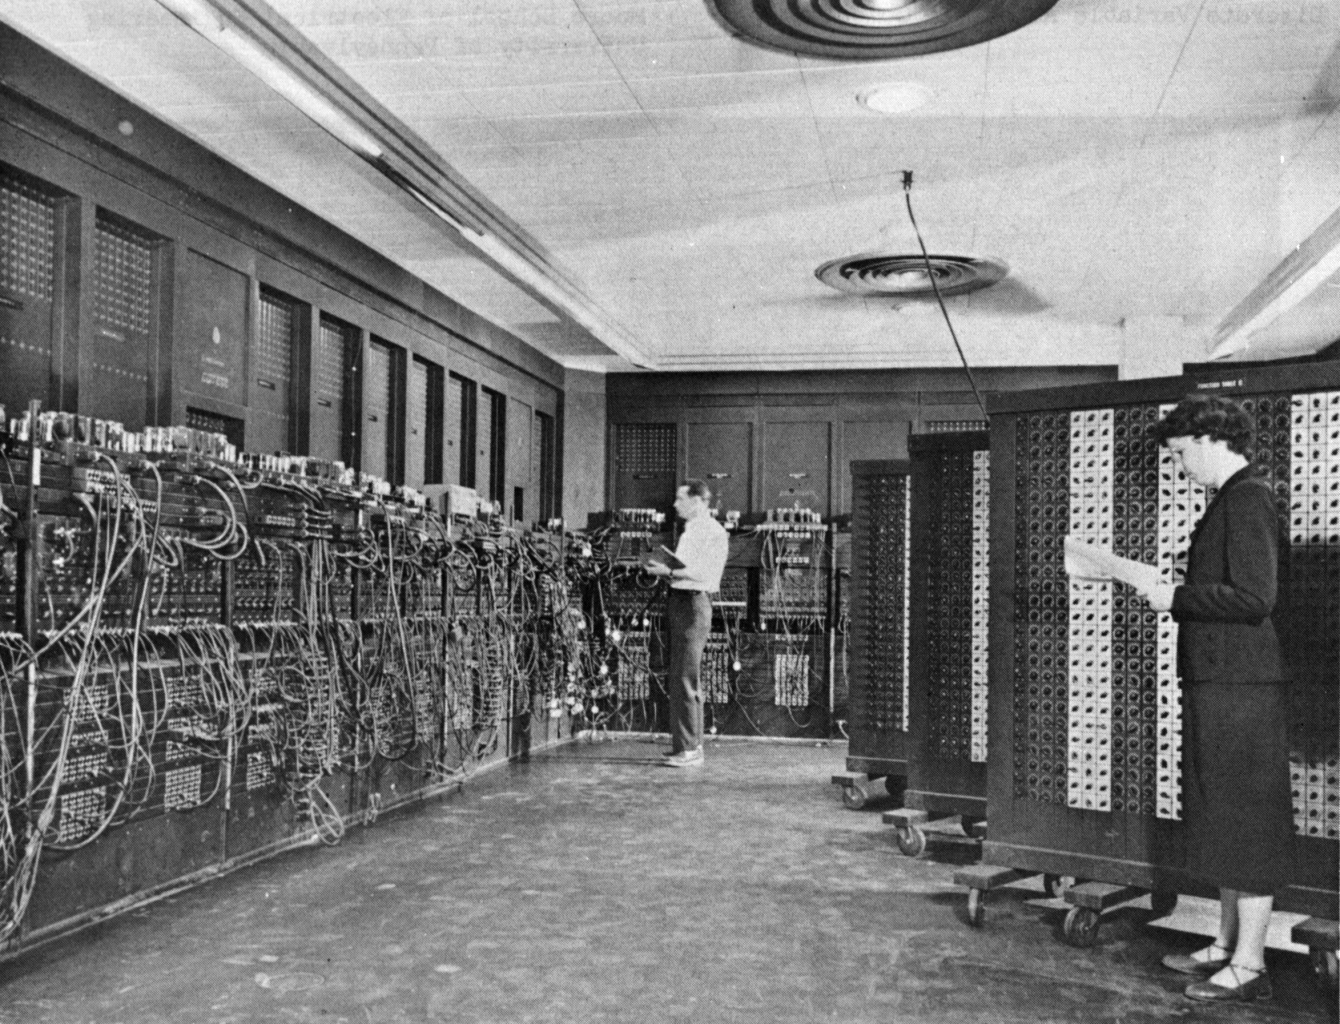
\includegraphics[height=6.5cm]{Eniac.jpg}}
  \end{figure}
\end{frame}
\begin{frame}
  \frametitle{История}
  \begin{figure}[t]
    \centering
    \subfigure[Fat Man]{
    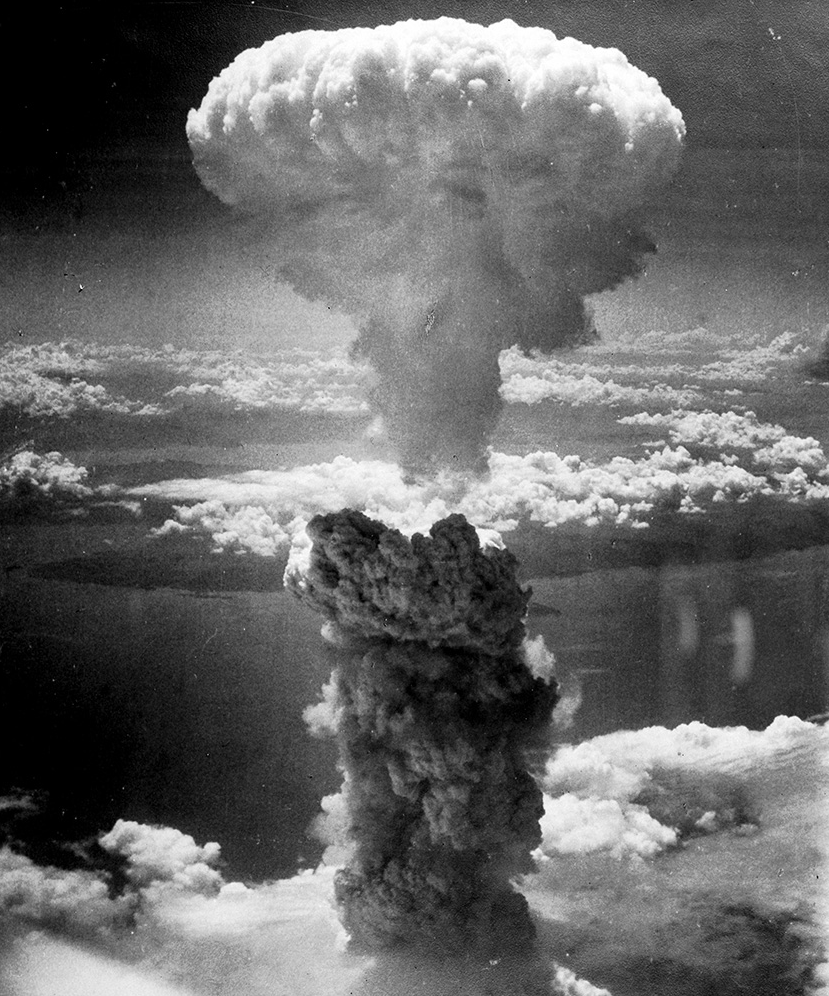
\includegraphics[height=6.5cm]{fatman.png}}
  \end{figure}
\end{frame}

\lstset{language=C++,
        basicstyle=\ttfamily,
        keywordstyle=\color{green}\ttfamily,
        stringstyle=\color{red}\ttfamily,
        commentstyle=\color{blue}\ttfamily,
        morecomment=[l][\color{magenta}]{\#}
}
\begin{frame}[fragile]
\frametitle{Монте Карло - Дефиниция}
\pause
\begin{lstlisting}
RandomGenerator rng;
for (int i = 0; i < nSamples; i++) {
   x   = sample(rng, ..);
   res = compute(x, ..);
   accumulate(res);
}
reportResults();
\end{lstlisting}
\end{frame}

\begin{frame}[fragile]
\frametitle{Пример}
\pause
\begin{lstlisting}
RandomGenerator rng;
int hits = 0;
for (int i = 0; i < nSamples; i++) {
   float x = rng.getUniform();
   float y = rng.getUniform();
   int res = x*x + y*y < 1.0f ? 1 : 0;
   hits += res;
}
float final = hits * 4.0f / nSamples;
\end{lstlisting}
\end{frame}

\begin{frame}
  \frametitle{$\pi$ - Монте Карло}
  uncomment the code to show animation
%  \begin{figure}[t]
%    \animategraphics[height=7.5cm,loop,autoplay]{2}{pi_frame-}{0}{9}
%  \end{figure}
\end{frame}

\begin{frame}
  \frametitle{$\pi$ - Монте Карло}
  \begin{equation*}
   h(x,y) = \begin{cases}
        1,& \text{ако } x^2 + y^2 < 1 \\
        0,& \text{иначе}\\
        \end{cases}
  \end{equation*}
  \pause

  \begin{equation*}
    \Omega = x \in [0 .. 1] \times y \in [0 .. 1]
  \end{equation*}
  \pause

  \begin{equation*}
   \int_{\Omega} h(x,y) dx dy = \frac{\pi}{4} \Rightarrow 
  \end{equation*}
  \pause
  \begin{equation*}
   \pi = 4 \int_{\Omega} h(x,y) dx dy
  \end{equation*}
\end{frame}


\begin{frame}
  \frametitle{Монте Карло интегриране}
  \begin{equation*}
  I = \int_{\Omega} f(\mathbf{x}) d \mathbf{x}, \quad
  x \in \mathbb{R}^d,  \quad
  V = \int_{\Omega} d \mathbf{x}
  \end{equation*}
  \pause
  \begin{equation*}
  Q_N = V \frac{1}{N} \sum_{i=1}^N f(\mathbf{x_i}) = V \overline{\mathbf{f}}, \quad 
  \mathbf{x_1}, \mathbf{x_2}, \dots,  \mathbf{x_N} \in \Omega
  \end{equation*}
  \pause
  \begin{equation*}
  \mathrm{Var} (f) = \sigma_N^2 = \frac{1}{N-1} \sum_{i=1}^N (f(\mathbf{x_i}) - \overline{\mathbf{f}})^2
  \end{equation*}
  \pause

  \begin{equation*}
  \delta Q_N = \sqrt{\mathrm{Var}(Q_N)} = V \frac{\sigma_n} {\sqrt{N}}
  \end{equation*}

\end{frame}


\begin{frame}
  \frametitle{Сходимост}
%  \begin{figure}[t]
    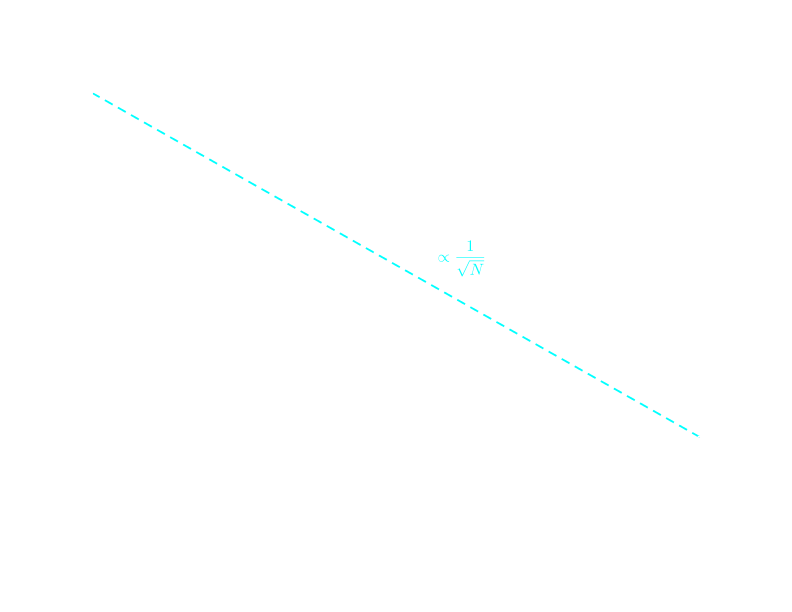
\includegraphics[height=8.0cm]{mc_error2.png}
%  \end{figure}
\end{frame}
\begin{frame}
  \frametitle{Сходимост}
  \begin{table}
  \begin{tabular}{l | c | c }
            &   1-D  &  S-D   \\
\hline \hline
Монте Карло & $\mathcal{O}(N^{-1/2})$    & $\mathcal{O}(N^{-1/2})$ \\ \pause 
Трапеците   & $\mathcal{O}(N^{-2})$      & $\mathcal{O}(N^{-2/s})$ \\ \pause
Симпсон     & $\mathcal{O}(N^{-4})$      & $\mathcal{O}(N^{-4/s})$ \\ 
%Квази МК    & $\mathcal{O}(log(n) n^{-1})$ & $\mathcal{O}(log(n)^s n^{-1})$ \\
\end{tabular}
%\caption{Сходимост на методи за числено интегриране}
\end{table}
\end{frame}



\begin{frame}
  \frametitle{Математика}
  \textbf{Вероятност}
  \begin{equation*}
      P(A) = \frac{|A|}{|A| + |!A|}
  \end{equation*}
  \pause
  \textbf{Разпределение}
  \begin{itemize}
  \item \textbf{Кумулативна функция}
  \begin{equation*}
      P(X < x) = F(x) \in [0..1]
  \end{equation*}
  \pause
  \item \textbf{Плътност}
  \begin{equation*}
      f(x) = \frac{dF(x)}{dx} \pause
  \end{equation*}
  \end{itemize}
\end{frame}

\begin{frame}
  \frametitle{Математика}
  \textbf{Униформно разпределение}
  \begin{itemize}
  \item \textbf{Плътност}
  \begin{equation*}
    f(x)= 
        \begin{cases}
        1,& \text{ако } x \in [0..1)\\
        0,& \text{иначе}
        \end{cases}
  \pause
  \end{equation*}
  \item \textbf{Кумулативна функция}
  \begin{equation*}
    F(x)= 
        \begin{cases}
        0,& x \in (-\infty, 0) \\
        x,& x \in [0..1)\\
        1,& x \in [1, -\infty) \\
        \end{cases}
  \end{equation*}
  \pause
  \end{itemize}
\end{frame}




\begin{frame}
  \frametitle{Математика}
  \textbf{Гаусово разпределение}
  \begin{itemize}
  \item \textbf{Плътност}
  \begin{equation*}
      f(x) = \frac{1}{\sigma \sqrt{2 \pi}} e^{-\frac{(x-\mu)^2}{2\sigma^2}} \pause
  \end{equation*}
  \item \textbf{Кумулативна функция}
  \begin{equation*}
      F(x) = \frac{1}{2} [1 + erf(\frac{x-\mu}{\sigma\sqrt{2}})] \pause
  \end{equation*}
  \end{itemize}
\end{frame}


\begin{frame}
  \frametitle{Mandelbrot set}
%  \begin{figure}[t]
    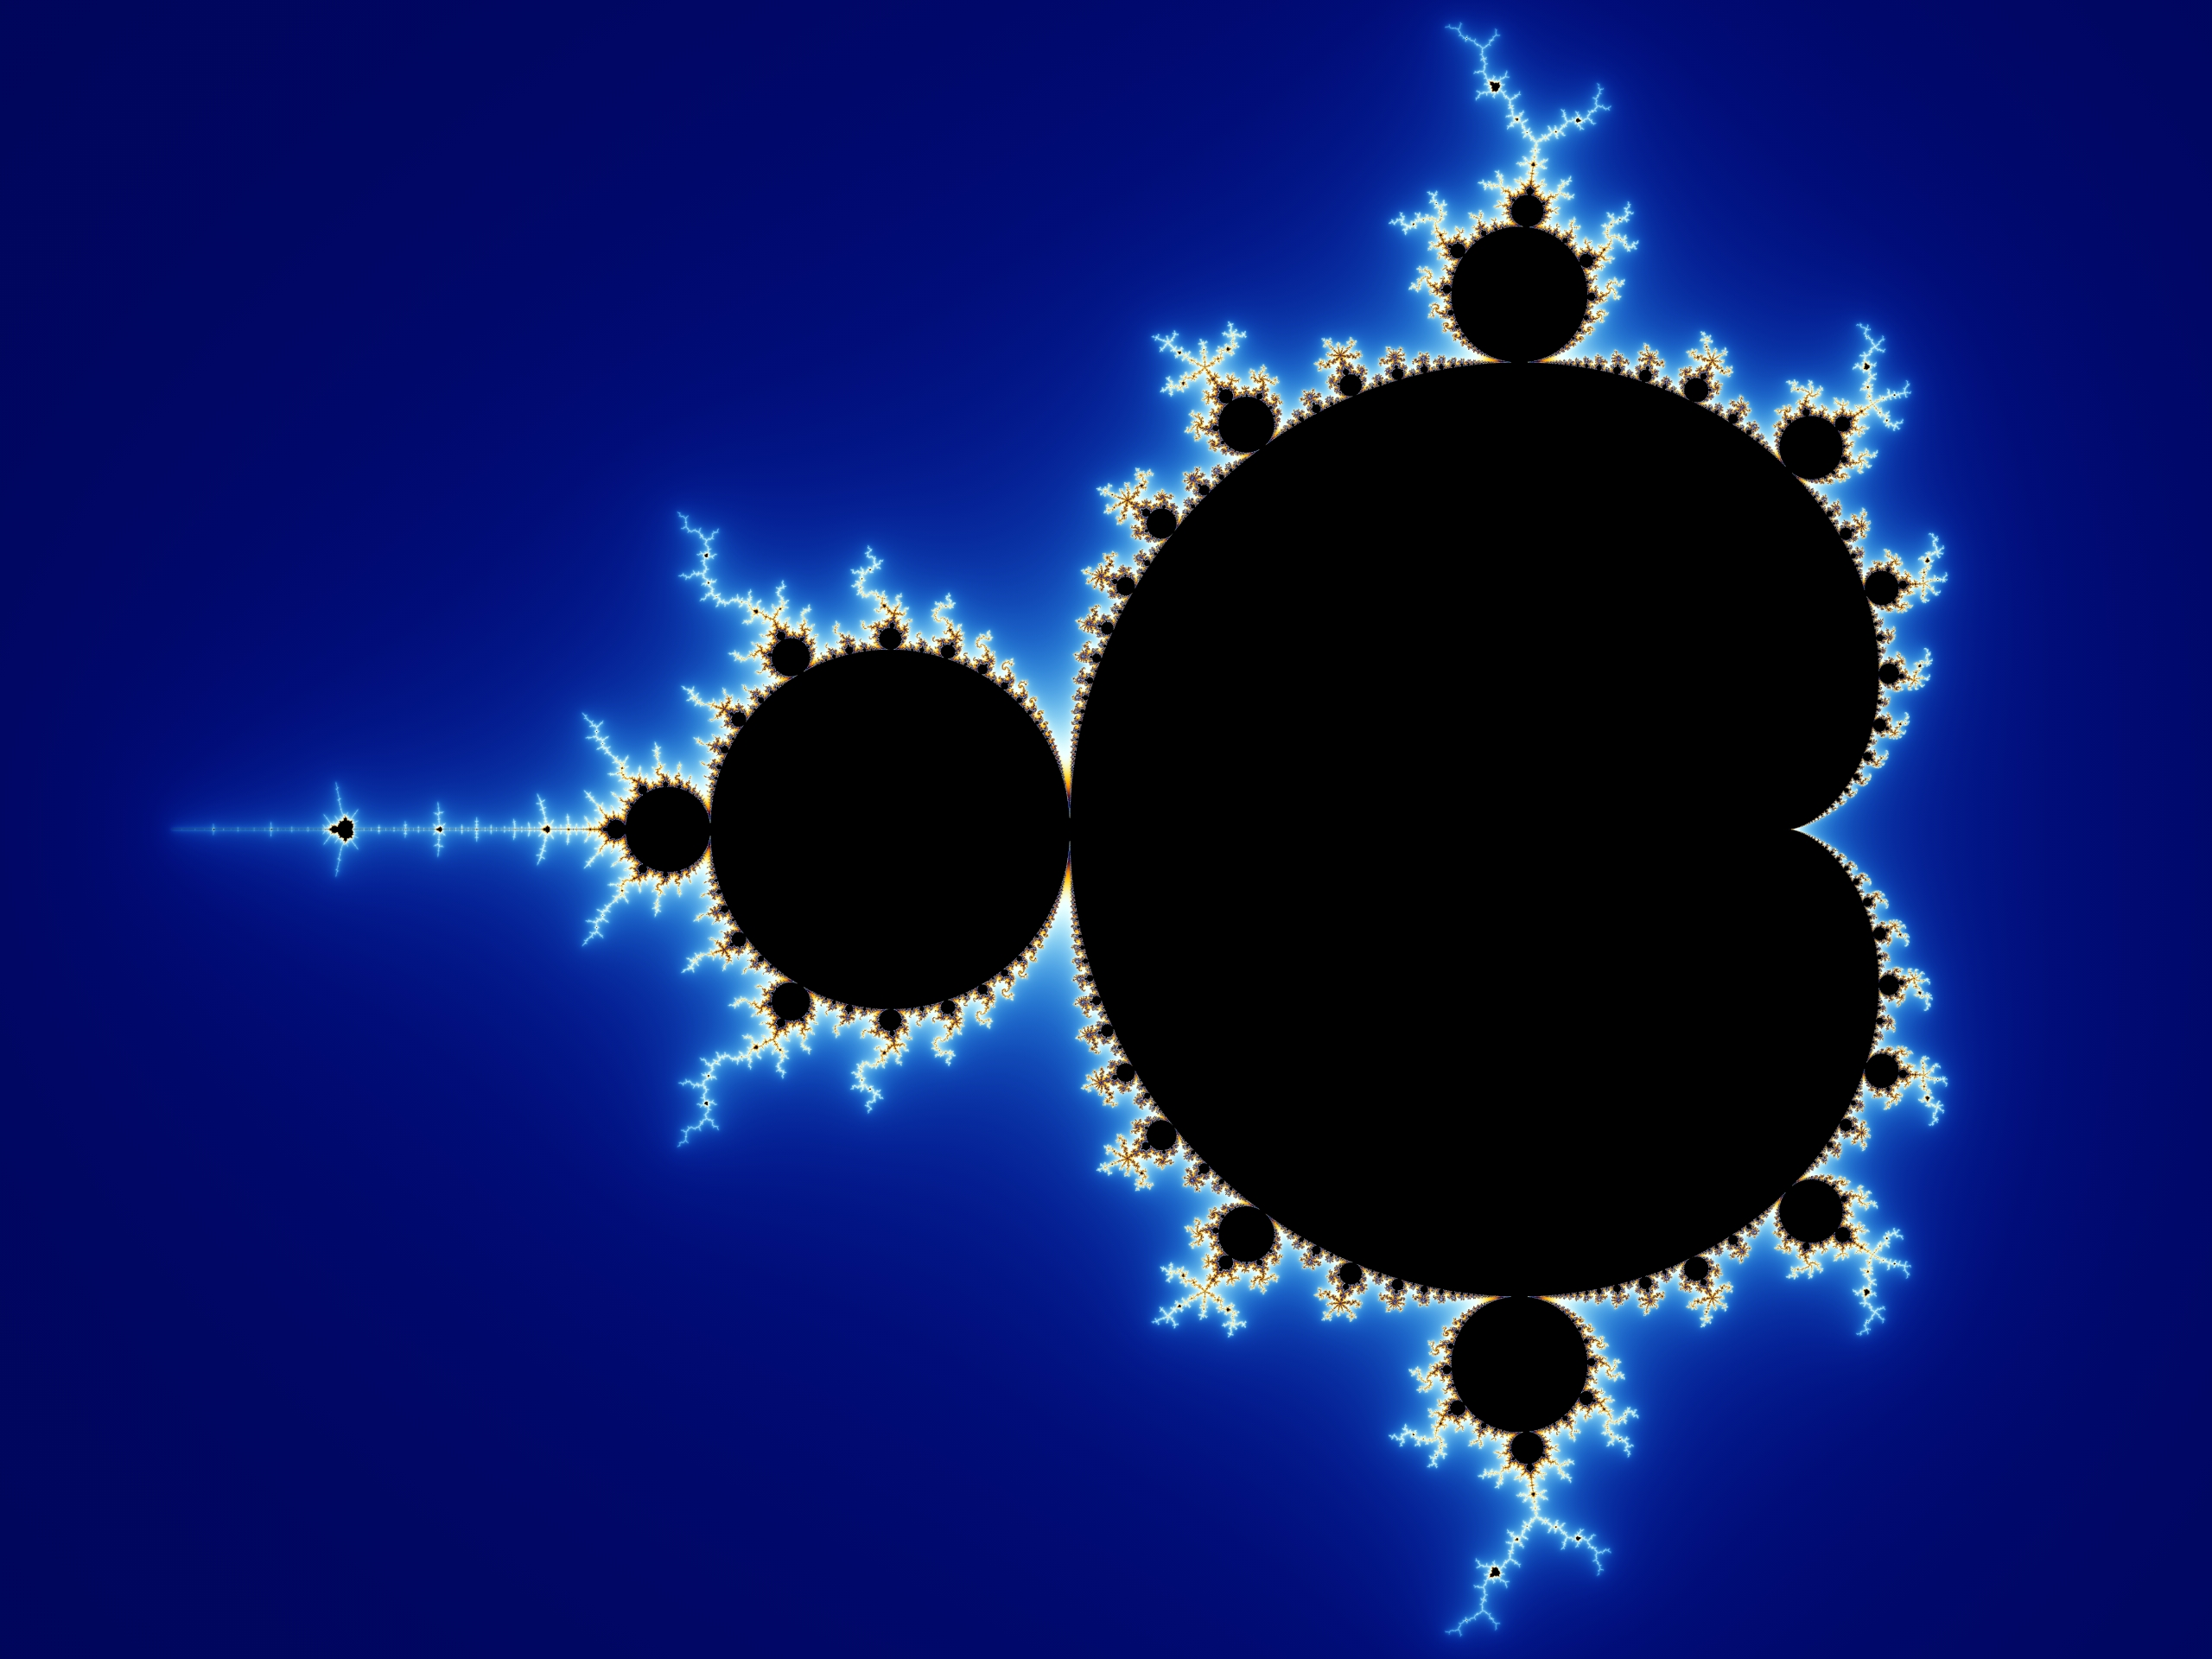
\includegraphics[height=8.0cm]{Mandel_zoom_00_mandelbrot_set.jpg}
%  \end{figure}
\end{frame}

\begin{frame}
  \frametitle{Недостатъци на Монте Карло}
  \pause
  Защото работи\pause
  \begin{itemize}
  \item с ограничени ресурси\pause
  \item върху сложни проблеми\pause
  \item в истинският свят\pause
  \item без алтернатива
 %leave out the \pause on the final item
  \end{itemize}
\end{frame}
%\section{Main Body} % add these to see outline in slides

\begin{frame}
  \frametitle{Математика}
  Писането на уравнения е лесно
  \begin{itemize}
  \item Просто ги копирайте от статията\pause
  \item или си ги напишете на ръка
    \begin{equation*}
      \textbf{p}^* = \underset{\textbf{p}}{\arg\!\min}~\sum_{\textbf{x}}\left[ I(\textbf{W}(\textbf{x};\textbf{p})) - T(\textbf{x}) \right]^2
    \end{equation*}
  \end{itemize}
\end{frame}

\begin{frame}
  \frametitle{Секси картинки}
  \begin{figure}[t]
    \centering
    \subfigure[материал 1]{
    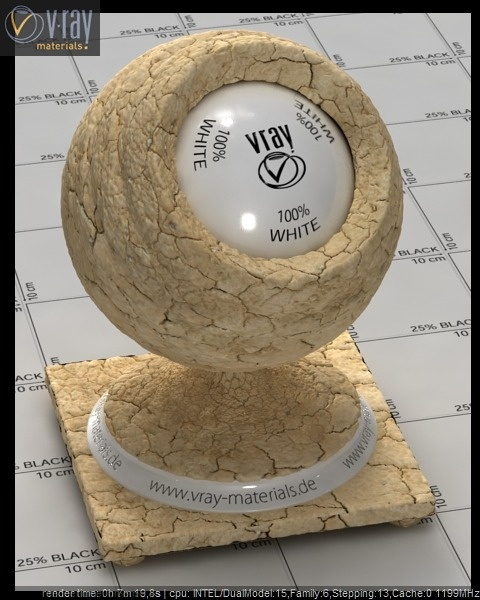
\includegraphics[width=3.2cm]{mat1.jpg}}
    \subfigure[друг материал]{
    
\includegraphics[width=3.2cm]{mat2.jpg}}
    \subfigure[още един]{
    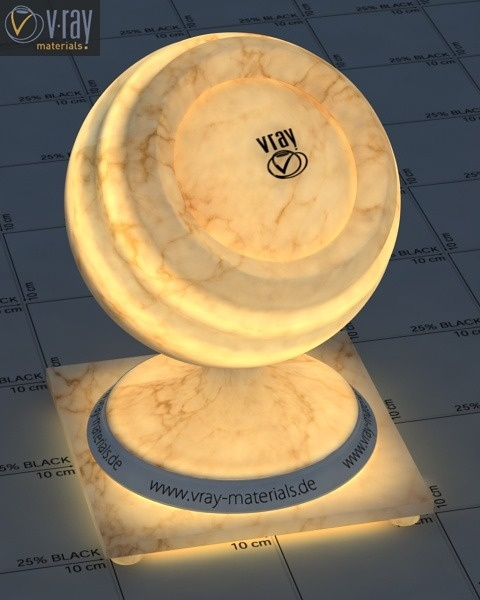
\includegraphics[width=3.2cm]{mat3.jpg}}
  \end{figure}
\end{frame}

\begin{frame}
  \frametitle{Филмче}
   Това не съм го пробвал дали работи.
  \begin{center}
    \movie[height=5cm,width=6.5cm,poster,autostart,loop]{}{leaves.avi}
  \end{center}
  \begin{itemize}
  \item Movies only seem to work in Adobe Reader
  \item Movie file is not embedded, it must be on the computer
  \end{itemize}
\end{frame}

%\section{Conclusion} % add these to see outline in slides

\begin{frame}
  \frametitle{Разни линкове}
  \begin{itemize}
  \item https://github.com/ymadzhunkov/cg2\_2015.git
%  \item Brought to you by www.shawnlankton.com
%  \item Please let me know about improvements!
%  \item This was supposed to look like a KeyNote Show
%  \item inspiration: http://www.ucl.ac.uk/~ucbpeal/latexposter.html
%  \item inspiration: http://newsgroups.derkeiler.com/... (in code)
        %http://newsgroups.derkeiler.com/Archive/Comp/comp.text.tex/2007-11/msg00299.html
  \end{itemize}
\end{frame}

\begin{frame}
  \frametitle{Въпроси}
\end{frame}
\end{document}
